\documentclass[conference]{IEEEtran}
\IEEEoverridecommandlockouts
% The preceding line is only needed to identify funding in the first footnote. If that is unneeded, please comment it out.
\usepackage{cite}
\usepackage{amsmath,amssymb,amsfonts}
\usepackage{algorithmic}
\usepackage{graphicx}
\usepackage{textcomp}
\usepackage[utf8]{inputenc}
\usepackage{hyperref}
\usepackage{amsthm, amssymb,amsmath}
\usepackage{mathrsfs}
\usepackage{mathtools}
\usepackage{pgfplots}
\usepackage{todonotes}
\usepackage{dsfont}
\usepackage{enumitem}
\usepackage[capitalise,nameinlink]{cleveref}
\usetikzlibrary{shapes}


\renewcommand{\:}{\mathrel{\coloneqq}}
\renewcommand{\=}{\ensuremath{\eqqcolon}}
\renewcommand{\epsilon}{\varepsilon}
\usepackage[caption=false, font=normalsize, labelfont=sf, textfont=sf]{subfig}
\newcommand{\dd}{\ensuremath{\,\mathrm{d}}}
\newcommand{\ddt}{\ensuremath{\tfrac{\dd}{\dd t}}}

\newcommand{\R}{\ensuremath{\mathbb{R}}}
\newcommand{\N}{\ensuremath{\mathbb{N}}}

\newcommand{\rr}{\text{r}}
\newcommand{\nr}{\text{nr}}

\date{\today}
\newtheorem{Definition}{Definition}
\newtheorem{Routing}{Routing}
\newtheorem{Results}{Results}
\newtheorem{Lemma}{Lemma}
\newtheorem{Corollary}{Corollary}
\newtheorem{Assumption}{Assumption}

\newtheorem{Remark}{Remark}
\newtheorem{Example}{Example}
\newtheorem{Theorem}{Theorem}
\newtheorem{Challenge}{Challenge}
\newtheorem{Proposition}{Proposition}

\newcommand{\0}{\ensuremath{\boldsymbol{0}}}
\newcommand{\A}{\mathcal{A}}
\newcommand{\V}{\mathcal{V}}
\newcommand{\C}{\mathcal{C}}
\newcommand{\cS}{\mathcal{S}}
\newcommand{\T}{\mathcal{T}}

\newcommand{\fR}{\mathfrak{R}}
\newcommand{\fRD}{\mathfrak{RD}}
\newcommand{\fRL}{\mathfrak{RL}}
\newcommand{\fRU}{\mathfrak{RU}}


\newcommand{\source}{\mathcal O}
\newcommand{\sink}{\mathcal D}
\newcommand{\OD}{\source\sink}
\newcommand{\Aout}{\mathcal{A}_{\textnormal{out}}}
\newcommand{\Ain}{\mathcal{A}_{\textnormal{in}}}
\newcommand{\vout}{v_{\text{tail}}}
\newcommand{\vin}{v_{\text{head}}}
\newcommand{\paths}{\mathcal{P}}
\newcommand{\bx}{\boldsymbol{x}}
\newcommand{\bg}{\boldsymbol{g}}
\newcommand{\bu}{\boldsymbol{u}}
\newcommand{\btau}{\boldsymbol{\tau}}
\newcommand{\btheta}{\boldsymbol{\theta}}
\newcommand{\bb}{\boldsymbol{b}}
\newcommand{\bh}{\boldsymbol{h}}
\newcommand{\bk}{\boldsymbol{k}}
\newcommand{\bm}{\boldsymbol{m}}
\newcommand{\bp}{\boldsymbol{p}}
\newcommand{\bs}{\boldsymbol{s}}
\newcommand{\bX}{\boldsymbol{X}}
\newcommand{\app}{\text{r}}
\newcommand{\napp}{\text{nr}}
\newcommand{\shortp}{\mathcal{Y}}
\newcommand{\ord}{\boldsymbol{\text{Ord}}}
\newcommand{\e}{\mathrm{e}}
\DeclareMathOperator*{\argmin}{arg\,\min}
\newcommand{\ext}{\textbf{\textnormal{ext}}}


\newcommand{\Id}{\mathrm{Id}}
\newcommand{\bcX}{\boldsymbol{\mathcal{X}}}
\newcommand{\Int}{\ensuremath{\int\limits}}

\newcommand{\len}{\textnormal{len}}
\newcommand{\todoAll}[1]{\todo[inline,color=red!30!yellow]{All: #1}}
\begin{document}

\title{A software framework for solving dynamic traffic assignment\\
{\footnotesize \textsuperscript}
\thanks{Identify applicable funding agency here. If none, delete this.}
}

\author{\IEEEauthorblockN{First author given Name Surname}
\IEEEauthorblockA{\textit{dept. name of organization (of Aff.)} \\
\textit{name of organization (of Aff.)}\\
City, Country \\
email address}}

\maketitle

\begin{abstract}
\end{abstract}

\begin{IEEEkeywords}
\end{IEEEkeywords}

\section{Introduction}
 In recent years, dynamic traffic assignment (DTA) has gained heightened interest, as researchers and practitioners are recognizing the need to predict the spatio-temporal evolution of traffic and the limitations of  static traffic assignment methods\cite{peeta2001foundations}. Existing static planning methods cannot fully model traffic congestion in road networks because of their inability to represent departure/arrival traveler's decisions and queue formation and dissipation when traffic demand exceeds road capacities\cite{nie2010solving}. They were developed for long term transportation planning and are not applicable in dynamic route guidance systems that require the ability to solve transportation problems in real time\cite{boyce1989route}.
 
Though the theory of DTA is still relatively undeveloped, variational inequality (VI) has proven to provide a unified formulation to address various classes of equilibrium and equivalent optimization problems in the DTA context. VI formulations can model more realistic traffic scenario by bypassing the issues of solution intractability in DTA problems with asymmetric link interactions associated with other analytical DTA methods such as mathematical programming and optimal control formulations . In addition, VI's extension and sensitivity analysis can be conveniently performed \cite{peeta2001foundations}. In this paper, we extend VI formulation to unify analytical DTA models with simulation-based DTA models. Simulation-based DTA methods compliment analytical techniques by addressing the shortcomings of analytical link models and exit functions in reproducing dynamic traffic interactions, satisfying First-In-Fist-Out property, and replicating complex vehicles and multi-user class interactions.

Using this general DTA VI formulation, we created a modular and extendable software framework, \textit{ta\_solver} to solve DTA problems. There exist many commercial and scientific DTA software tools that uses simulation-based models such as CONTRAM \cite{taylor2003contram}, DTALite \cite{zhou2014dtalite}, Dynameq \cite{mahut2010traffic}, DynaMIT-P \cite{DynaMIT,ben2001dynamit}, DYNASMART-P \cite{DYNASMART,mahmassani2004dynasmart}, DynusT \cite{chiu2011dynust}, INTEGRATION \cite{rakha2012integration}, and TransDNA \cite{TransDNA}. To the best of our knowledge, our software is first to combine simulation-based DTA models with analytical methods including mathematical programming and optimal control into one software platform, using a clear underlying VI DTA formulation. The general VI formulation determines the overall software architecture, but also provide a way to incorporate any type of DTA problem that can be represented with VI. Ziliaskopoulos and Waller developed VISTA, a internet-based geographic information system that integrates transportation spatio-temporal data and models into a single framework. While VISTA does integrate analytical and simulation-based DTA models and DTA solution algorithms, it was built with particular focus on the integration of different transportation modules, unlike \textit{ta\_solver} that was designed to solve DTA problems. In addition, VISTA has no fundamental DTA problem formulation, while \textit{ta\_solver} is based on VI. 

Hence, our papers contributions include:
\begin{enumerate}
    \item A clear and unified variational inequality formulation for traffic assignment problems (with good notation).
    \item A modular software framework,\textit{ta\_solver},  with solvers based on the unified variational inequality formulation.
    \item Demonstration of the performance of the software framework using different models.
\end{enumerate}

\section{Variational Inequality for DTA}

\section{Software Framework Description}

\begin{figure}[h]
    \centering
    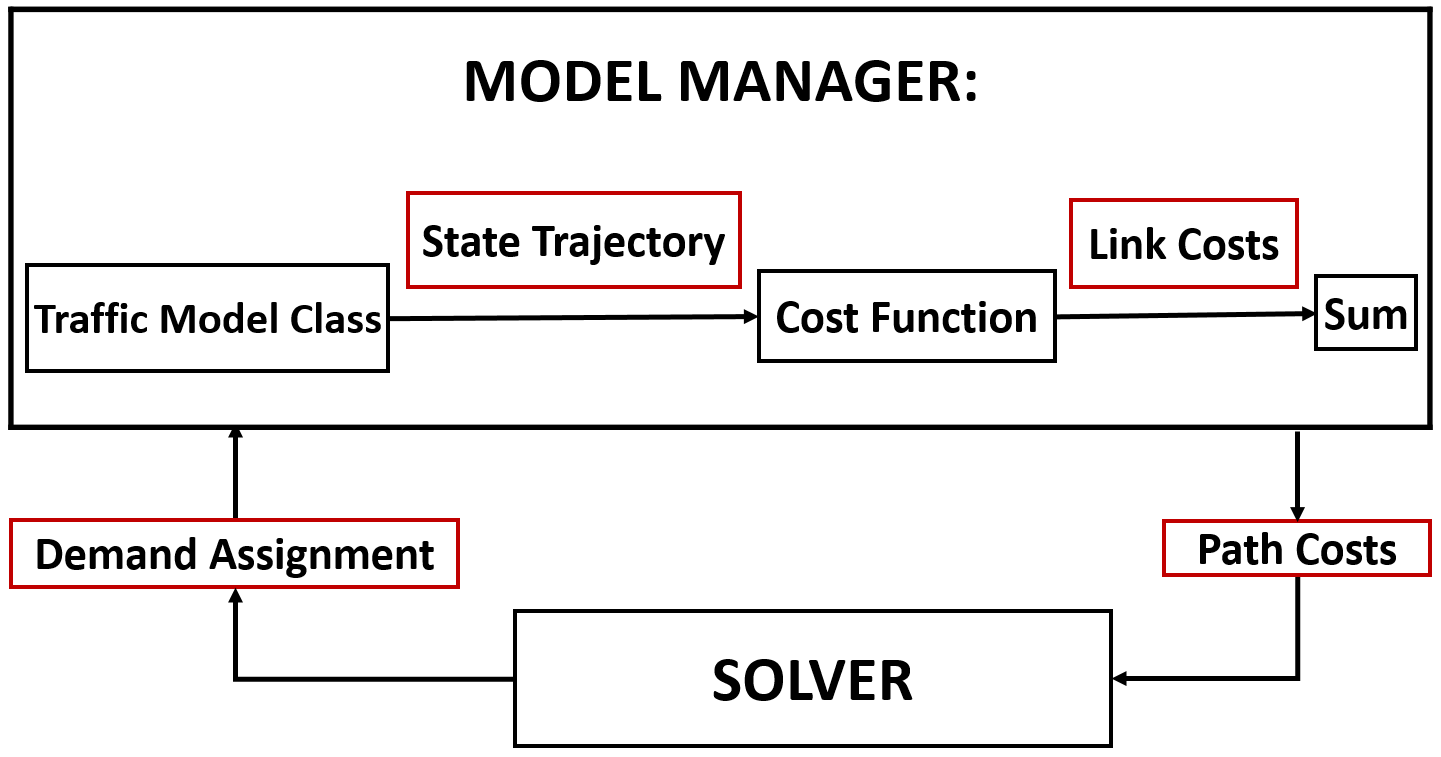
\includegraphics[width=\linewidth]{Software_Block_Diagram.PNG}
    \caption{Software Framework Architecture}
    \label{fig:Block_Diagram}
\end{figure}

Using the unified VI DTA formulation, we designed a modular and extendable software framework to solve DTA problems. As shown in Figure~\ref{fig:Block_Diagram}, the software framework has two main modules: the Model Manager and the Solver modules. The Demand Assignment and Path Costs components are wrappers for an assignment per path, commodity and time, and for path travel costs respectively.

The Model Manager has three components that correspond to the $F = \Sigma\circ c \circ \mathbb{T}$ composition function: the Traffic Model, Cost Function and Sum components. The State Trajectory module is a wrapper for the link states (e.g: flow per link), and the Link Cost module is a wrapper for the travel cost per link (e.g experienced travel time on a link). The Model Manager's role is to translate an assignment $h$, specified as a sequence of demand per path by the Demand Assignment module, into the corresponding path costs, represented as a sequence of cost per path.

The Solver module serves as an interface to plug in solution algorithms for DTA. The generic SOLVER works in a loop in which it generates candidate demand assignments, and expects to be given the corresponding network path costs. This loop continues until an equilibrium demand assignment is reached. 

The advantage of our modular software framework is that it can be easily extended to address different DTA problems. The Traffic Model and Cost Function components interfaces enable a user to plug in different traffic models and cost functions to address diverse DTA problems. For example, the software framework currently include three traffic models: the static model, Merchant and Nemhauser (MN) model, and the Point Queue Model, which all integrate in the framework via the Traffic Model component. The framework has a travel time based cost function. A user can add an energy or emission based cost function. The Solver interface allows to incorporate different DTA solution algorithm. We included three solver algorithms: the Method of Successive Averages, the Frank-Wofle Algorithm, and the Extra Projection Methods, which can be applied depending on the $F$ function properties. Finally, we also designed the whole Model Manager component as an interface, enabling a user to integrate an implementation of the $F$ composition function without having to use the Traffic model, Cost Function and Sum modules. This is useful for problems, such as simulaton-based DTA problems, where the traffic model is tightly coupled with the cost function evaluation. The complete documentation on software framework, with installations instructions can be found at ...

\section{Implemented Traffic Models}
\subsection{Static Model}
\subsection{MN Model}
\subsection{Point Queue Model}

\section{Implemented Algorithms}

\subsection{Method of Successive Averages}
The Method of Successive Averages (MSA) is a heuristic-based algorithm and does not put any restriction on $F$. However, it does not guarantee convergence to the optimal solution for the general VI problem \cite{nie2010solving}. MSA is used to initialize the other algorithms. The algorithm's steps are described below:
\begin{enumerate}
    \item Start with a feasible assignment $h^1$ and set $k=1$.
    \item Calculate the all-or-nothing assignment $y^k$.
    \item If ${\frac {\langle F(h^k),y^k-x^k \rangle} {\langle y^k, F(x^k)\rangle}} \leq
    \epsilon$, stop. Otherwise, go to step 4.
    \item set $\alpha = 1/k$, and $h^{k+1} = (1-\alpha)h^k + \alpha y^k$. 
    \item Set $k = k+1$ and go back to step 2.
\end{enumerate}

\subsection{Frank-Wolfe Algorithm}
The Frank-Wolfe Algorithm (FW) applies when $F$ is convex and continuously differentiable \cite{fukushima1984modified,gartner1977analysis}. It has the following steps:
\begin{enumerate}
\item Start with a feasible assignment $h^1$, obtained using the Method of Successive Averages. Set $k=1$.
\item Determine the all-or-nothing assignment $y^k$ given the current assignment $h^k$.
\item Terminate if $\nabla F(h^k)(h^k-y^k) \leq \epsilon$ stop; otherwise, go to step 4.
\item Calculate $d^k = y^k - h^k$
\item Set $h^{k+1} = h^k +\alpha d^k$, where $\alpha$ is a solution the one-dimensional problem: $\min_{0 \leq \alpha \leq 1}G(h^k + \alpha d^k)$ and $G = \int_h F$.
\item Set $k = k+1$ and go back to step 2.
\end{enumerate}

\subsection{Extra Projection Method}
The Extra Projection Method (EPM) is based on the Euclidean Projection define as $\Pi_\mathcal{H} = argmin\{\lVert h-h^0\rVert:h \in\mathcal{H} \}$ and $\lVert.\rVert$ is the Euclidean norm. The EPM guarantees convergence when $F$ is Lipschitz continuous and pseudo monotone \cite{nie2010solving}. The EPM steps are described below:
\begin{enumerate}
\item Start with a feasible assignment $h^1$, obtained using the Method of Successive Averages. Set $k=1$.
\item If ${\frac {\langle F(h^k),y^k-x^k \rangle} {\langle y^k, F(x^k)\rangle}} \leq \epsilon$, where $y^k$ is the all-or-nothing assignment, then stop. Otherwise, go to step 3.
\item Find $z^k = \Pi_\mathcal{H}(h^k - \tau F(h^k))$, , where $\tau < L$ and $L$ is the Lipschitz constant for $F$.
\item Find $h^{k+1} = \Pi_\mathcal{H}(h^k - \tau F(z^k))$, where $\tau$ is a above.
\item Set $k = k+1$ and go back to step 2.
\end{enumerate}

Since $L$ can be difficult to predetermine in practice, \cite{nie2010solving} propose the following algorithm to update $\tau$ after obtaining solution $h^{k+1}$:
\begin{enumerate}
    \item Evaluate $\phi(h^{k+1})$ and $\phi(h^k)$, where $\phi(h)$ is the all-or-nothing assignment given $h$.
    \item if $\phi(h^{k+1})-\phi(h^k) < 0$ and $\frac{|\phi(h^{k+1})-\phi(h^k)|}{|\phi(h^k)|}> \epsilon$, set $\tau = \tau \times \sigma$, where $\epsilon$ and $\sigma$ are positive scalars between 0 and 1.
\end{enumerate}

\section{Numerical Results}

\section{Conclusions}\label{sec:concl}

\section*{Acknowledgment}


\bibliographystyle{alpha}
\bibliography{citation.bib}

\end{document}
